\newpage

\anonchapter{Лабораторная работа №6}
\setcounter{chapter}{6}

\begin{center}
Изучение поглощения света в полупроводниках\\
(4 часа)
\end{center}

\section{Цель работы}
Целью работы является изучения основных механизмов поглощения света в полупроводниках и освоение методики исследований спектров поглощения света в полупроводниках в видимой и ближней инфракрасной области спектра.

\section{Теоретическая часть}
\subsection{Коэффициент поглощения света}
Если поток фотонов с длиной волны $\lambda$ и интенсивностью $I_{0}(\lambda)$ падает на плоскопарралельный образец толщиной $d$, то можно исследовать интенсивность отражённого от поверхности образца света $I_{R}(\lambda)$ и определить безразмерный коэффициент отражения

\begin{equation}
R(\lambda) = \frac{I_{R}(\lambda)}{I_{0}(\lambda)}
\end{equation}

а также измерить интенсивность прошедшего через образец света $I_{T}(\lambda)$ и определить безразмерный коэффициент пропускания

\begin{equation}
T(\lambda) = \frac{I_{T}(\lambda)}{I_{0}(\lambda)}
\end{equation}

Интенсивность прошедшего через образец света однозначно определяется коэффициентом отражения, поглощением внутри образца и отражением от внутренних граней. Закон Бугера-Ламберта внутри образца, на поверхность которого падает свет выглядит следующим образом:

\begin{equation}
I(x, \lambda) = I_{0}(\lambda) \left[ 1 - R(\lambda) \right] \exp{(- \alpha (\lambda) x )}
\end{equation}
где $\alpha(\lambda)$ - коэффициент поглощения, имеет размерность обратной длины.

Величина $\alpha^{-1}$ определяет толщину кристалла, проходя через которую свет ослабляется в $e$ раз. Это значит, что можно считать величину $\alpha$ вероятностью поглощения фотона на единице длины. Если имеется несколько незвисимых механизмов поглощения света в кристалле, то полный коэффициент поглощения будет суммой коэффициентов, определяемых каждым механизмом независимо.

\begin{equation}
\alpha(\lambda) = \sum\limits_{i}{\alpha_{i}(\lambda)}
\end{equation}

Зависимость $\alpha(\lambda)$ называется спектром поглощения для данного вещества.

Практическое использование формулы Бугера-Ламберта приводит к известным проблемам, связанным с невозможностью прямого имзмерения интенсивности света внутри кристалла на определённой глубине. При измерении интенсивности света, прошедшего через образец толщиной $d$ необходимо учитывать не только поглощение света данным слоем, но также долю отражённого света и сумму всех потоков с учётом многократного отражения. Сумму всех потоков можно представить в виде бесконечной геометрической прогрессии, первый член которой равен $I_{0} (1-R)^2 \exp(-\alpha d)$, а множитель $R^2 \exp(-2 \alpha d)$. Интенсивность света, прошедшего через обрезец $I_{T}$, таким образом находится как

\begin{equation}
I_{T} = I_{0} \frac{(1-R)^2 \exp(-\alpha d)}{1 - R^2 \exp(-2 \alpha d)}
\end{equation}

Если учесть, что обычно $\alpha d \gg 1$, в знаменателе можно пренебречь вторым членом и считать

\begin{equation}
I_{T} = I_{0} (1-R)^2 \exp(-\alpha d)
\end{equation}

Откуда можно получить коэффициент поглощения на данной длине волны:

\begin{equation}
\alpha = \frac{1}{d} \ln \frac{I_{0} (1-R)^2}{I_{T}}
\end{equation}

Если неизвестен коэффициент отражения, то величину $\alpha$ можно определить, сравнивая интенсивность света, прошедшего через два образца из одного материала с одинаковой обработкой поверхностью, но различной толщины. В таком случае для образцов с толщинами $d_{1}$ и $d_{2}$

\begin{equation}
\alpha = \frac{1}{d_{1}-d_{2}} \ln \frac{I_{T1}}{I_{T2}}
\end{equation}

\subsection{Механизмы поглощения света}
Основные механизм поглощения света в полупроводниках определяются возможными типами переходов носителей заряда между зонами, или типами возбуждаемых светом тепловых колебаний решётки кристалла (фононов). Электронные и дырочные механизмы поглощения схематически показаны на рисунке \ref{pic6_transition}.

\begin{figure}[h!]\centering
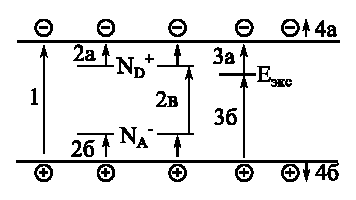
\includegraphics[height=6cm]{pic6_transition.eps}
\caption{Схема электронных переходов при различных механизмах поглощения света}
\label{pic6_transition}
\end{figure}

На рисунке обозначены:

\begin{enumerate}
\item Собственное или фундаментальное поглощение света, связанное с переходом электрона из валентной зоны в зону проводимости.
\item примесное поглощение, связанное с переходами электронов с примесного уровня в зону проводимости (2а на рисунке), из валентной зоны на примесный уровень (2б) или между различными примесными центрами (2в).
\item Экситонное поглощение, связанное с возбуждением экситона (переход 3б) или распадом на пару электрон-дырка (3а).
\item Поглощение свободными носителями заряда, сопровождаемое переходом свободных носителей на более выоские энергетические состояния внутри зоны.
\item Фононное поглощение (на рисунке не может быть отражено), связанное с возбуждением в кристалле одного или нескольких фононов - квантов тепловых колебаний решётки.
\end{enumerate}

Рассмотрим форму спетра поглощения для каждого из механизмов по отдельности.

\subsubsection{Собственное поглощение}
Рассмотрим поглощение фотона с энергией $E_{\text{ф}} = \hbar \omega$ непрямозонным полупроводником с шириной запрещённой зоны $E_{g} < E_{\text{ф}}$. Пусть зонная структура имеет вид, приведённый на рисунке \ref{pic6_zone}.

\begin{figure}[h!]\centering
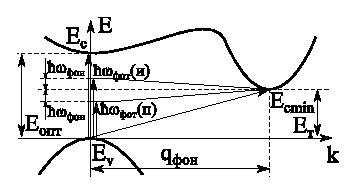
\includegraphics[height=6cm]{pic6_zone.eps}
\caption{Схема непрямых переходов электронов при собственном поглощении}
\label{pic6_zone}
\end{figure}

